% pdflatex mf_ex1.tex
\documentclass{beamer}
\usepackage[latin1]{inputenc}
\usepackage{graphicx}
\usepackage{beamerthemesplit}
\usepackage{multicol,pgf,tikz}
\usetikzlibrary{shapes,arrows}
\usepackage{multimedia}
\usepackage{hyperref}
\usepackage{color}
\input{epsf}

\definecolor{durham}{cmyk}{0.5,0.8,0.,0.6}
%\setbeamercovered{transparent}
\mode<presentation>
{  \usetheme[height=7mm]{Rochester}
  \usecolortheme[named=durham]{structure}
  \useinnertheme[shadow]{rounded}
  \usefonttheme[onlymath]{serif}
  %\setbeamercovered{transparent}
  \setbeamertemplate{blocks}[rounded][shadow=true]
  \setbeamertemplate{navigation symbols}{} 
  %\setbeamertemplate{footline}{\hspace{12cm} \insertframenumber/\inserttotalframenumber
  \setbeamertemplate{footline}{V. Gonzalez-Perez \hspace{10.2cm} \insertframenumber/\inserttotalframenumber }
}

%%%%%%%%%%%%%%%%
\newcommand{\lcdm}{$\rm{\Lambda CDM}$}
\newcommand{\gl}{\textsc{galform}}
\newcommand{\eg}{\textsc{eagle}}
\newcommand{\egdm}{\textsc{eagleDMO}}
\newcommand{\lgl}{\textsc{l-galaxies}}
\newcommand{\subf}{\textsc{subfind}}
\newcommand{\msun}{{\rm M}_{\odot}}
\newcommand{\mb}{M_{\rm Break}}
\newcommand{\mth}{{\rm M}_{200}^{\rm crit}}
\newcommand{\mtry}{\todo[\textcolor{blue}{Upd.}]}
\newcommand{\stry}{\todo[\textcolor{blue}{From Shaun: Upd.}]}
\newcommand{\ptry}{\todo[\textcolor{blue}{From Peter: Upd.}]}
\newcommand{\nm}{$\langle N \rangle_{M}$}
%%%%%%%%%%%%%%%%

\title{Python, SQL and  the  mass function.}
\author{{\bf Violeta Gonzalez-Perez}}
\institute{@violegp\\
}
\date{}


\begin{document}
\frame{\titlepage 
\vspace{-0.5cm}
\begin{center}
\includegraphics[height=0.25\textheight]{/home/violeta/charlas/fig/logos/icg-logo.pdf}
\end{center}
}



%%_____Flow charts_____________________________________
\tikzstyle{decision} = [diamond, draw=green!50!black!50,fill=green!50!black!50, text centered, text width=3.8em]
\tikzstyle{up} = [rectangle, draw, very thick,
draw=blue!50!black!50,level distance=4cm,
    text width=15em, text centered, rounded corners, minimum height=8em]
\tikzstyle{down} = [rectangle, draw, very thick,
draw=red!50!black!50,level distance=4cm,
    text width=5em, text centered, rounded corners, minimum height=3em]
\tikzstyle{up1} = [rectangle, draw, very thick,
draw=blue!50!black!50,level distance=4cm,
    text width=5em, text centered, rounded corners, minimum height=5em]
\tikzstyle{down1} = [rectangle, draw, very thick,
draw=red!50!black!50,level distance=4cm,
    text width=5em, text centered, rounded corners, minimum height=5em]
\tikzstyle{up2} = [rectangle, draw, very thick,
draw=blue!50!black!50,level distance=4cm,
    text width=10em, text centered, rounded corners, minimum height=8em]
\tikzstyle{sed} = [rectangle, draw, very thick,
draw=green!50!black!50,level distance=4cm,
    text width=5em, text centered, rounded corners, minimum height=7em]
\tikzstyle{thing} = [rectangle, draw, very thick,
draw=red!50!black!50,level distance=4cm,
    text width=4em, text centered, rounded corners, minimum height=2em]
\tikzstyle{line} = [draw, -latex]
\tikzstyle{cloud} = [draw, ellipse,fill=black]   
\tikzstyle{newm} = [draw=green!50!black!50, ellipse,fill=green!50!black!50,text width=4em,text centered]   
\tikzstyle{prop} = [circle,fill=red, level distance=1cm,text width=5em,text centered]   
\tikzstyle{empty} = [minimum height=2em]   


%%_____Introduction______________________________________

\begin{frame}{Observed galaxy stellar mass function}
\begin{center}
\includegraphics[width=1.4\textwidth]{/home/violeta/charlas/fig/course/baldry12data.jpg}
\end{center}
% wget http://www.astro.ljmu.ac.uk/~ikb/research/data/gsmf-B12.txt
\end{frame}

\begin{frame}{Starting with python}
\begin{itemize}
\item A place to start: \url{https://docs.python.org/3/tutorial/}
\item Jupyter notebooks: \url{http://jupyter.org/}
\item Plotting with python: \url{http://matplotlib.org/index.html}
\end{itemize}
\begin{center}
\includegraphics[width=1.\textwidth]{/home/violeta/charlas/fig/course/python0.jpg}
\end{center}
\end{frame}


\begin{frame}{A program in python}
\begin{center}
\includegraphics<1>[width=1.\textwidth]{/home/violeta/charlas/fig/course/loop1.jpg}

\includegraphics<2>[width=1.\textwidth]{/home/violeta/charlas/fig/course/loop2.jpg}
\end{center}
\end{frame}


\begin{frame}{Reading and plotting in python}
\begin{center}
\includegraphics[width=1.2\textwidth]{/home/violeta/charlas/fig/course/py_read_plot.jpg}
\end{center}
{\bf Exercise 1:} Write a program that plots and saves as a pdf the GSMF from Baldry+12, including error bars and in log scales in both axis and units M($M_{\odot}h^{-1}$) and $\Phi(\rm{Mpc}^{-3}h^{3}/dlog\rm{M})$.
\end{frame}


\begin{frame}{The Millennium simulation}
\begin{center}
\includegraphics[height=0.7\textheight]{/home/violeta/charlas/fig/intro/virgo.jpg}

\url{http://www.virgo.dur.ac.uk/}
\end{center}
\end{frame}

\begin{frame}{The milliMillennium}
\begin{center}
\url{http://virgodb.cosma.dur.ac.uk:8080/Millennium/}
\end{center}
\begin{itemize}
\item milliMillennium box size = $62.5$ Mpc$h^{-1}$ \\
\item Mass of each dark matter particle = $8.6\cdot 10^8$M$_{\odot}h^{-1}$
\item There are different tables with information on the DM only simulations and also on galaxy models used to populate it.
\includegraphics[height=0.7\textheight]{/home/violeta/charlas/fig/course/snap1.jpg}
\end{itemize}
\end{frame}


\begin{frame}{A basic Structured Query Language (SQL) query}
SQL is a computer language for storing, manipulating and retrieving data stored in relational database.

\includegraphics<1>[width=1.\textwidth]{/home/violeta/charlas/fig/course/snap2.jpg}
\includegraphics<2>[width=1.\textwidth]{/home/violeta/charlas/fig/course/snap3.jpg}
\end{frame}

\begin{frame}{A query to get information on the DM haloes}
\begin{center}
\includegraphics[height=0.7\textheight]{/home/violeta/charlas/fig/course/snap2.jpg}
\end{center}
{\bf Exercise 2:} Starting from the 'Demo queries' H1, get all the haloes in the milimillennium including their number of particles and a measure of mass. Save the result into a file.
\end{frame}

\begin{frame}{A halo mass function (HMF) from your SQL query}

{\bf Exercise 3:} Calculate the (HMF) from the milliMillennium in 2 ways. {\tiny Box size = $62.5$ Mpc$h^{-1}$, m$_{DM}=8.6\cdot 10^8$M$_{\odot}h^{-1}$.} What happens if you use a different bin size? Make use of np.histogram and of: \includegraphics[height=0.8\textheight]{/home/violeta/charlas/fig/course/py_skip.jpg}
\end{frame}

\begin{frame}{The halo mass function: different mass definitions}
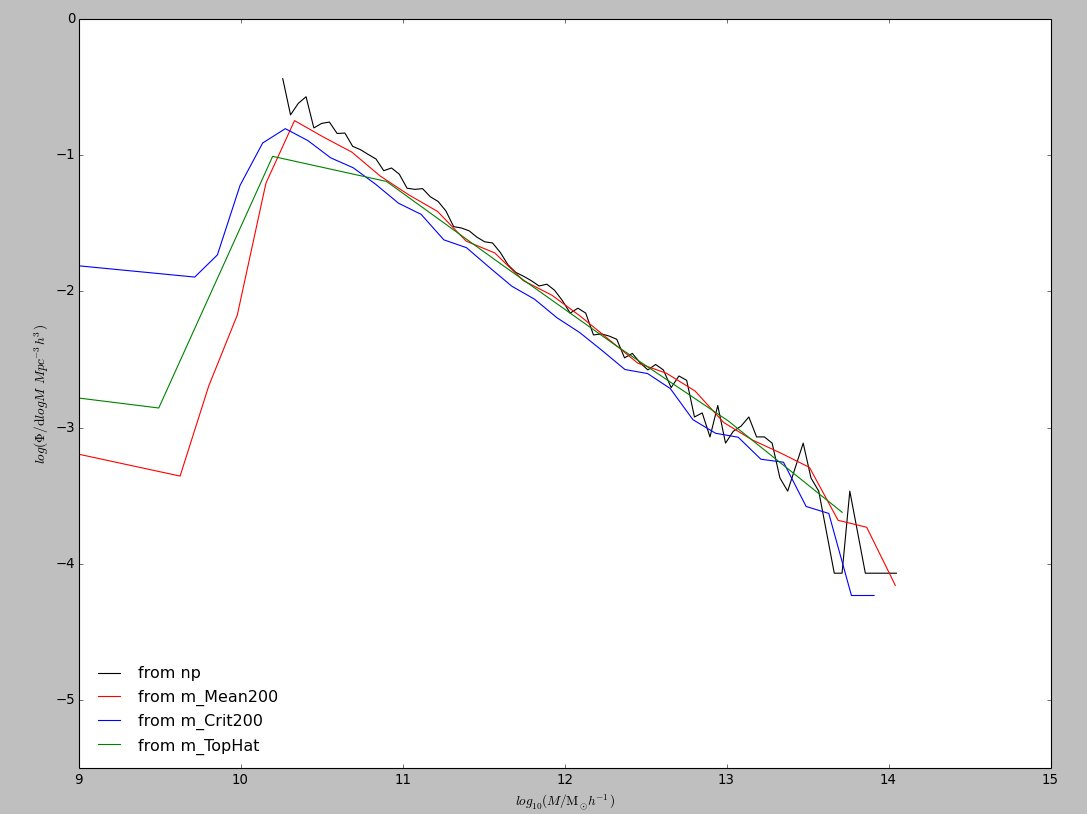
\includegraphics[height=0.9\textheight]{/home/violeta/charlas/fig/course/mf_masses.jpg}

{\small Knebe+15 lists halo mass definitions used in different galaxy models.}
\end{frame}


\begin{frame}{A SQL query for getting directly the HMF}
\texttt{\color{blue} select .1*(.5+floor((log10(m\_Crit200)+10.)/.1)) as mass, \\
log10(count(*)/power(62.5,3.)/.1) as phi \\
from millimil..MPAHalo \\
where snapnum$=63$ and m\_Crit200$>0.$ \\
group by $.1*(.5+$floor((log10(m\_Crit200)$+10.)/.1))$ \\ 
order by mass
}

\vspace{1cm}

{\bf Exercise 4:} Plot the HMF you obtain from the query above together with the 2 previous ones.
\end{frame}

\begin{frame}{The halo mass function: two types of queries}
\begin{center}
\includegraphics[height=0.9\textheight]{/home/violeta/charlas/fig/course/mf_queries.jpg}
\end{center}
\end{frame}


\begin{frame}{An SQL query from python}

{\bf Exercise 5:}
\begin{enumerate} 
\item Get John Helly's module with useful functions:\\ {\small \color{blue} \texttt{> wget http://icc.dur.ac.uk/Eagle/Database/eagleSqlTools.py}} 

\item Make a simple query. {\small When the URL points at the milli-millennium the username and password are ignored.}

\includegraphics[width=1.\textwidth]{/home/violeta/charlas/fig/course/myMillennium_sql.jpg}

\item The result is a numpy record array. Access the columns of the result with expressions like data["snapnum"], data["redshift"] etc. The column names and types are in data.dtype.fields.

\item Now, get the milliMellinium haloes, {\color{green}'millimil.haloes.txt'} with their positions, peculiar velocities, mass, half mass radius and the variables: \texttt{haloID}, \texttt{firstHaloInFOFgroupId}.
\end{enumerate}
\end{frame}


\begin{frame}{The galaxy stellar mass function (GSMF)}

{\bf Exercise 6:} Compare the observed GSMF that you previously downloaded with 2 GSMF derived from the halo mass function, assuming:
\begin{enumerate}
\item That the ratio between halo and stellar mass is the baryonic fraction,$f_b = \Omega_{b,0}/\Omega_{m,0}=0.04/0.308$, such that: $M_{*}=M_{\rm halo}\cdot f_b$
\item That the formation of stars and galaxies is inefficient in such a way that: $M_{*}=\epsilon\cdot M_{\rm halo}\cdot f_b$ (choose $\epsilon$, such that the observed knee of the GSMF is recovered). {\color{green} TIP: Use np.interp()}.
\end{enumerate}
\end{frame}


\begin{frame}{The galaxy stellar mass function }
\begin{center}
\includegraphics[height=0.8\textheight]{/home/violeta/charlas/fig/course/gsmf_fb.jpg}
\end{center}
The shapes are very different! We need a better model to connect the luminouse matter to the dark one.
\end{frame}


\begin{frame}{Populating the Millennium with galaxies}
\begin{center}
\includegraphics[height=0.9\textheight]{/home/violeta/charlas/fig/course/myMillennium.jpg}
\end{center}
\end{frame}


\begin{frame}{The semi-analytical GSMF}

{\bf Exercise 7:} Get the GSMF for the De Lucia et al. 2006 model, which is a comprehensive model of galaxy formation and evolution:\\

{\color{blue}\texttt{from millimil..DeLucia2006a}}

Save it to a file using \texttt{np.savetxt} and plot it together with your previous theoretical GSMF and compared to Baldry et al. 2012 data.
\end{frame}


\begin{frame}{The GSMF from the milliMillennium}
\begin{center}
\includegraphics[height=1.\textheight]{/home/violeta/charlas/fig/course/myMillennium_gsmf.jpg}
\end{center}
\end{frame}


%\begin{frame}{The mean halo occupation distribution (HOD)}
%????????????????????????????/
%{\bf Exercise 6:} Make a plot with the mean halo occupation distribution, i.e., the mean number of galaxies per halo in a given halo mass bin. For this purpose modify the SQL query you have used to directly get the  (example)
%
%\includegraphics[width=1.\textwidth]{/home/violeta/charlas/fig/course/milli_hod.pdf}
%\end{frame}


\begin{frame}{Other ways of populating DM only simulations}
\begin{center}
\includegraphics[height=.9\textheight]{/home/violeta/charlas/fig/intro/Lagos.pdf}

{\tiny {\sc credit:} Claudia Lagos}
\end{center}
\end{frame}

\begin{frame}{Halotools: using abundance matching and HOD models}

{\bf Exercise 8:} Get halotools, \url{https://halotools.readthedocs.io/}

{\small The easiest ways to install \texttt{halotools} require either \texttt{pip} or \texttt{conda}, make sure you have them installed.


\vspace{0.5cm} If you encounter a problem related to the c compilers, try:\\
{\color{blue}\texttt{> sudo apt-get install python-dev}}
}

\vspace{0.5cm}Verify your installation:
\begin{center}
\includegraphics[width=1.\textwidth]{/home/violeta/charlas/fig/course/ht_verify.jpg}
\end{center}
\end{frame}


\begin{frame}{millimil as a halo catalogue in Halotools: variables}

{\bf Exercise 9:} Modify the following code such that

\begin{itemize} 
\item \texttt{ids} and \texttt{upid} are initialized as 2 integer arrays with the size of the number of haloes downloaded.
\item Store \texttt{haloID} into the long integer array \texttt{ids}.
\item If \texttt{firstHaloInFOFgroupId}=\texttt{haloID} set \texttt{upid}$=-1$, and to any other number otherwise.
\end{itemize}
\begin{center}
\vspace{-1cm}\includegraphics[width=1.1\textwidth]{/home/violeta/charlas/fig/course/ht_setup1.jpg}
\end{center}
\end{frame}

\begin{frame}{millimil as a halo catalogue in Halotools: arrays}

{\bf Exercise 9:} Pass the arrays you've previously created, fixing the following:
\begin{center}
\includegraphics[width=1.\textwidth]{/home/violeta/charlas/fig/course/ht_setup2.jpg}
\end{center}
\end{frame}

\begin{frame}{millimil populated with the Zheng+07 model}

In the Zheng+07, the NFWPhaseSpace class from Halotools requires knowledge of halo concentration to assign an intra-halo spatial distribution to the satellites. By default, the concentration of the actual halos in the catalog are used for this purpose. However, we haven't downloaded that attribute so to have satellites distributed according to an NFW profile, we need an analytical model for the concentration-mass relation, such as the one from Dutton \& Maccio 2014:

{\bf Exercise 10:} Try
\begin{center}
\includegraphics[width=1.1\textwidth]{/home/violeta/charlas/fig/course/ht_setup3.jpg}
\end{center}
\end{frame}

\begin{frame}{The mean HOD}

{\bf Exercise 11:} Compare the mean HOD from Halotools with that from De Lucia et al. 2006 model.
\end{frame}

%-----------------------------------------------
\end{document}
